\section{Suma de enteros en base uno}

\subsection{MT Determinista de 1 cinta}

\subsubsection*{Diseño propuesto}
El algoritmo de resolución es el siguiente:

\begin{itemize}
    \item Ciclo:
    \begin{enumerate}[1.]
        \item Comenzar desde la izquierda y desplazarse hata el extremo derecho.
        \item Si el último elemnto es un 1:
        \begin{enumerate}[1.]
            \item Borrarlo.
            \item Volver al extremo izquierdo.
            \item Añadir un 1 en la primera posición
        \end{enumerate}
        \item Si el último elemnto es un \$:
        \begin{enumerate}[1.]
            \item Borrarlo.
            \item Volver al extremo izquierdo.
            \item \textbf{Parar}.
        \end{enumerate}
    \end{enumerate}
\end{itemize}

El diseño de la máquina queda representado en la Figura \ref{fig:MT-1A}.

\begin{figure}[h]
    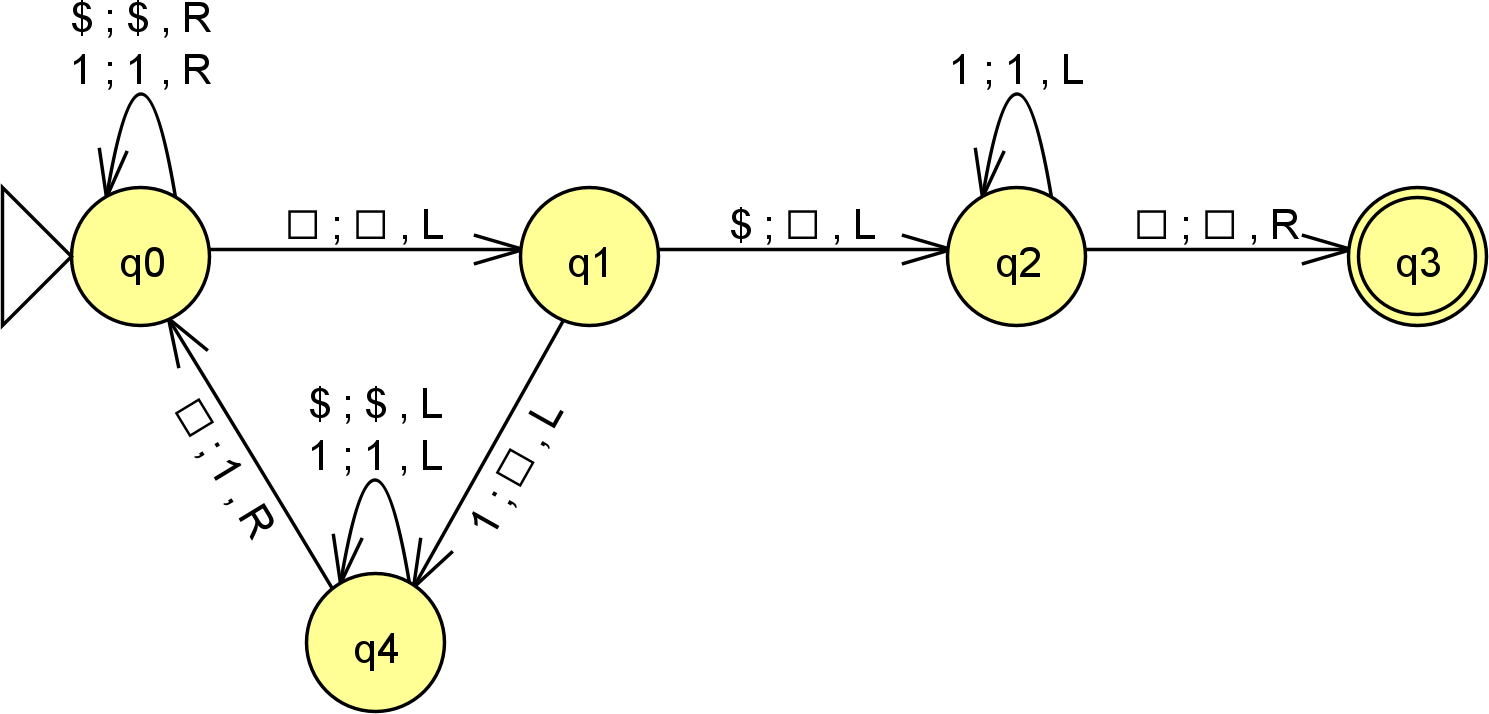
\includegraphics[width=\textwidth]{MT-1A.png}
    \caption{Implementación en JFLAP de MT-1A}
    \label{fig:MT-1A}
\end{figure}


\subsubsection*{Peor caso}
Dado que el formato de palabra que acepta la Máquina de Turing son dos conjuntos de 1 separados por el simbolo \$, el peor caso sería aquel en el que haya una mayor cantidad de 1 a la derecha del \$, ya que por cada 1 se requerirá una iteración para eliminarlo de la derecha y añadirlo en la izquierda, por lo que a más 1 más iteraciones serán necesarias.

\subsubsection*{Evaluación empírica}
Realizamos la evaluación empírica en el peor caso, tomando como $n_i$ el numero de 1 a la izquierda de \$, $n_d$ el número de 1 a la derecha de \$, y midiendo el número de pasos realizados para resolver el problema:

\begin{table}[h]
    \centering
    \begin{tabular}{lccc}
        Entrada & $n_i$ & $n_d$ & Pasos \\
        \hline
        $\lambda$               & 0  & 0  & N/A \\
        1\$                     & 1  & 0  & 6   \\
        \$1                     & 0  & 1  & 11  \\
        11\$                    & 2  & 0  & 8   \\
        \$11                    & 0  & 2  & 22  \\
        \$111                   & 0  & 3  & 37  \\
        \$1111                  & 0  & 4  & 56  \\
    \end{tabular}
\end{table}


\subsubsection*{Coste computacional}
Para obtener el coste computacional del algoritmo, aplicaremos Diferencias Finitas, basándonos en los datos de la evaluación empírica:




